\documentclass{beamer}

\usepackage{hyperref}
\usepackage{epstopdf} 
\usepackage{graphicx}
\usepackage{amssymb}

\title{Central Trigger Board}
\author{ Update \\ Jonathon Sensenig Nuno Barros}
\institute{University of Pennsylvania}
\date{}

% position the logo
%\addtobeamertemplate{frametitle}{}{%
%	\begin{textblock*}{100mm}(\textwidth,-1cm)
%		
\includegraphics[height=1cm,width=1cm,keepaspectratio]{figs/Penn-Shield.png}
%\end{textblock*}}

%Add page number to the foot bar
\expandafter\def\expandafter\insertshorttitle\expandafter{%
	\insertshorttitle\hfill%
	\insertframenumber\,/\,\inserttotalframenumber}

%Use an image as the background
%\usebackgroundtemplate{
%	
\includegraphics[width=\paperwidth,height=\paperheight]{figs/bblue3.pdf}
%

%Add logos to title page only
%\titlegraphic{
\includegraphics[width=1.75cm]{figs/DUNElogo_color.png}\hspace*{2.75cm}~
%	\includegraphics[width=3cm]{figs/shield-logotype-whitebkgd-RGB-4k.png}
%}

\usetheme{Copenhagen}
\setbeamertemplate{navigation symbols}{} %NO nav buttons!

% Color modification
\definecolor{MyBackground}{RGB}{234, 249, 255}
\definecolor{jgrey}{RGB}{121, 147, 179}
\definecolor{jred}{RGB}{181,0,0}
\setbeamercolor{background canvas}{bg=MyBackground}
\setbeamercolor{structure}{fg=jgrey}% to modify  immediately all palettes
\setbeamercolor{title}{fg=black}
\setbeamercolor{title in head/foot}{fg=jred}
\setbeamercolor{author}{bg=black,fg=white}
\setbeamercolor{frametitle}{fg=black}

\begin{document}
	\frame {
		\titlepage
		\hspace{0.2cm}
		
\includegraphics[width=10cm,height=2.25cm]{figs/dune_penn_logo.png}

	}
	\frame { %Page 1
		\frametitle{CTB Firmware}
			\framesubtitle{Brief reminder of the firmware design shown by Nuno at  DUNE collab. meeting. 
			\footnote{\href{https://indico.fnal.gov/event/14581/session/8/contribution/141/material/slides/0.pdf}{\textcolor{blue}{Link to full slides}}}	}
				\hspace{0.85cm} 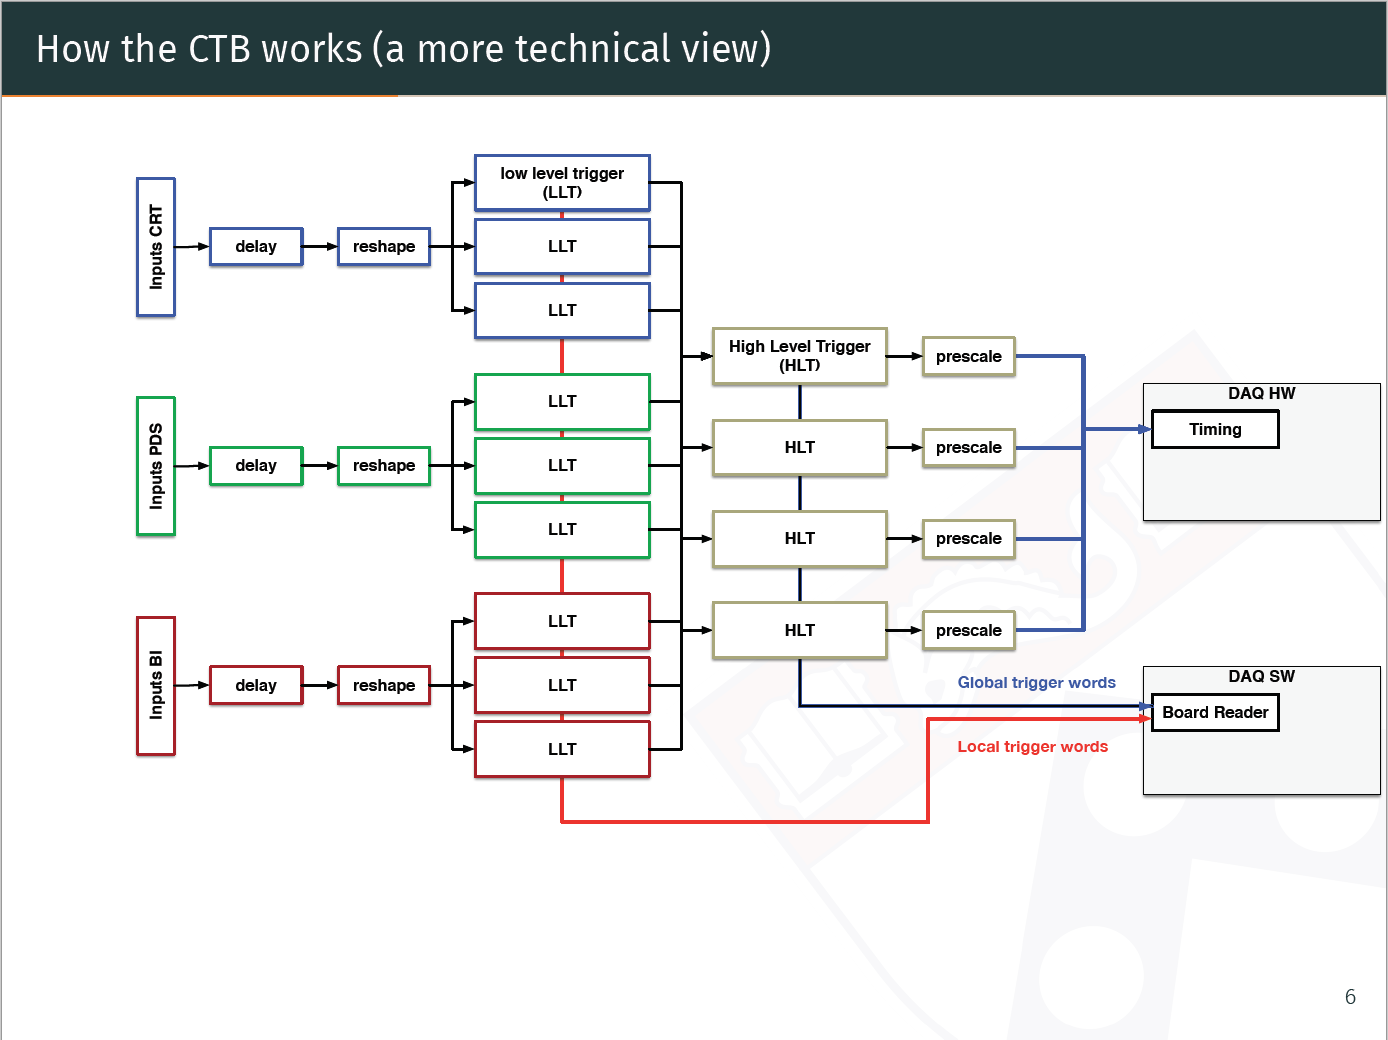
\includegraphics[width=9cm,height=6cm]{figs/ctb_func_collab.png}
	}
	\frame{  %Page 2
		\frametitle{Current firmware status}
			\framesubtitle{Firmware in place and tested.}	
				\includegraphics[width=11cm,height=5cm]{figs/ctb_curr_detail_2.png}	\\
				The latest (v1) firmware on the CTB.
	}
	\frame{  %Page 3
	    \frametitle{Upcoming firmware status 1/2}
	     \framesubtitle{Firmware which is near completion}
	     	\includegraphics[width=11cm,height=5cm]{figs/ctb_full_detail_2.png}\\
	     	\begin{itemize}
	     	\item[$\bullet$]The firmware under development. 
 			\item[$\bullet$] LLT = Low level trigger   and  HLT = High level trigger
	     	\item[$\bullet$]Note: There can be up to \textit{N} of the Low and High Level triggers.
   	     	\end{itemize}
	}

	\frame{  %Page 4
	\frametitle{Upcoming firmware status 2/2}
	\framesubtitle{What needs to be done, in words}

	\begin{itemize}
		\item[$\bullet$] Base configuration in place. Random triggers, timestamps.
		\item[$\bullet$] All the pieces in exist to do simple logic on inputs.
		\item[$\bullet$] These individual parts need to be put together (easy) and tested as a whole. Essentially the figure in the previous slide.
		\item[$\bullet$] Need to test sending triggers to timing board. 
		\item[$\bullet$] Will continue to develop trigger logic , i.e., LLT$\textunderscore$1 - LLT$\textunderscore$N and HLT$\textunderscore$1 - HLT$\textunderscore$N, as feedback and agreement on triggers progresses. 
	\end{itemize}
}
	\frame{  %Page X
	\frametitle{A Few More Trigger Details}	
	\begin{itemize}
		\item[$\bullet$]  Low Level Trigger (LLT) 
		\begin{itemize}
			\item[$\circ$] Forms a trigger based on inputs from a single subsystem
			\item[$\circ$] Never distributed to other systems as a trigger, but \textbf{is} recorded and sent to board reader.
			\item[$\circ$] Can be \textit{N} LLTs per susbsystem, in parallel
			\item[$\circ$] Configured from software at runtime.
		\end{itemize}
		\item[$\bullet$] High Level Trigger (HLT)
		\begin{itemize}
			\item[$\circ$] Configured from software at runtime.
			\item[$\circ$] Forms a trigger based on the LLT ouputs
			\item[$\circ$] Sent to the timing system for distribution to subsystems, also recorded and sent to board reader.
			\item[$\circ$] Can be prescaled on the CTB.
			\begin{itemize}				 
				\item[$\ast$] \textcolor{red}{Do we want to record prescaled HLTs?}
			\end{itemize}
			\item[$\circ$] Timing system can also veto HLTs	
		\end{itemize}	
	\end{itemize}
}

	\frame{  %Page 4
	\frametitle{CTB Data Words}
		\framesubtitle{The data packets sent from the PL}
			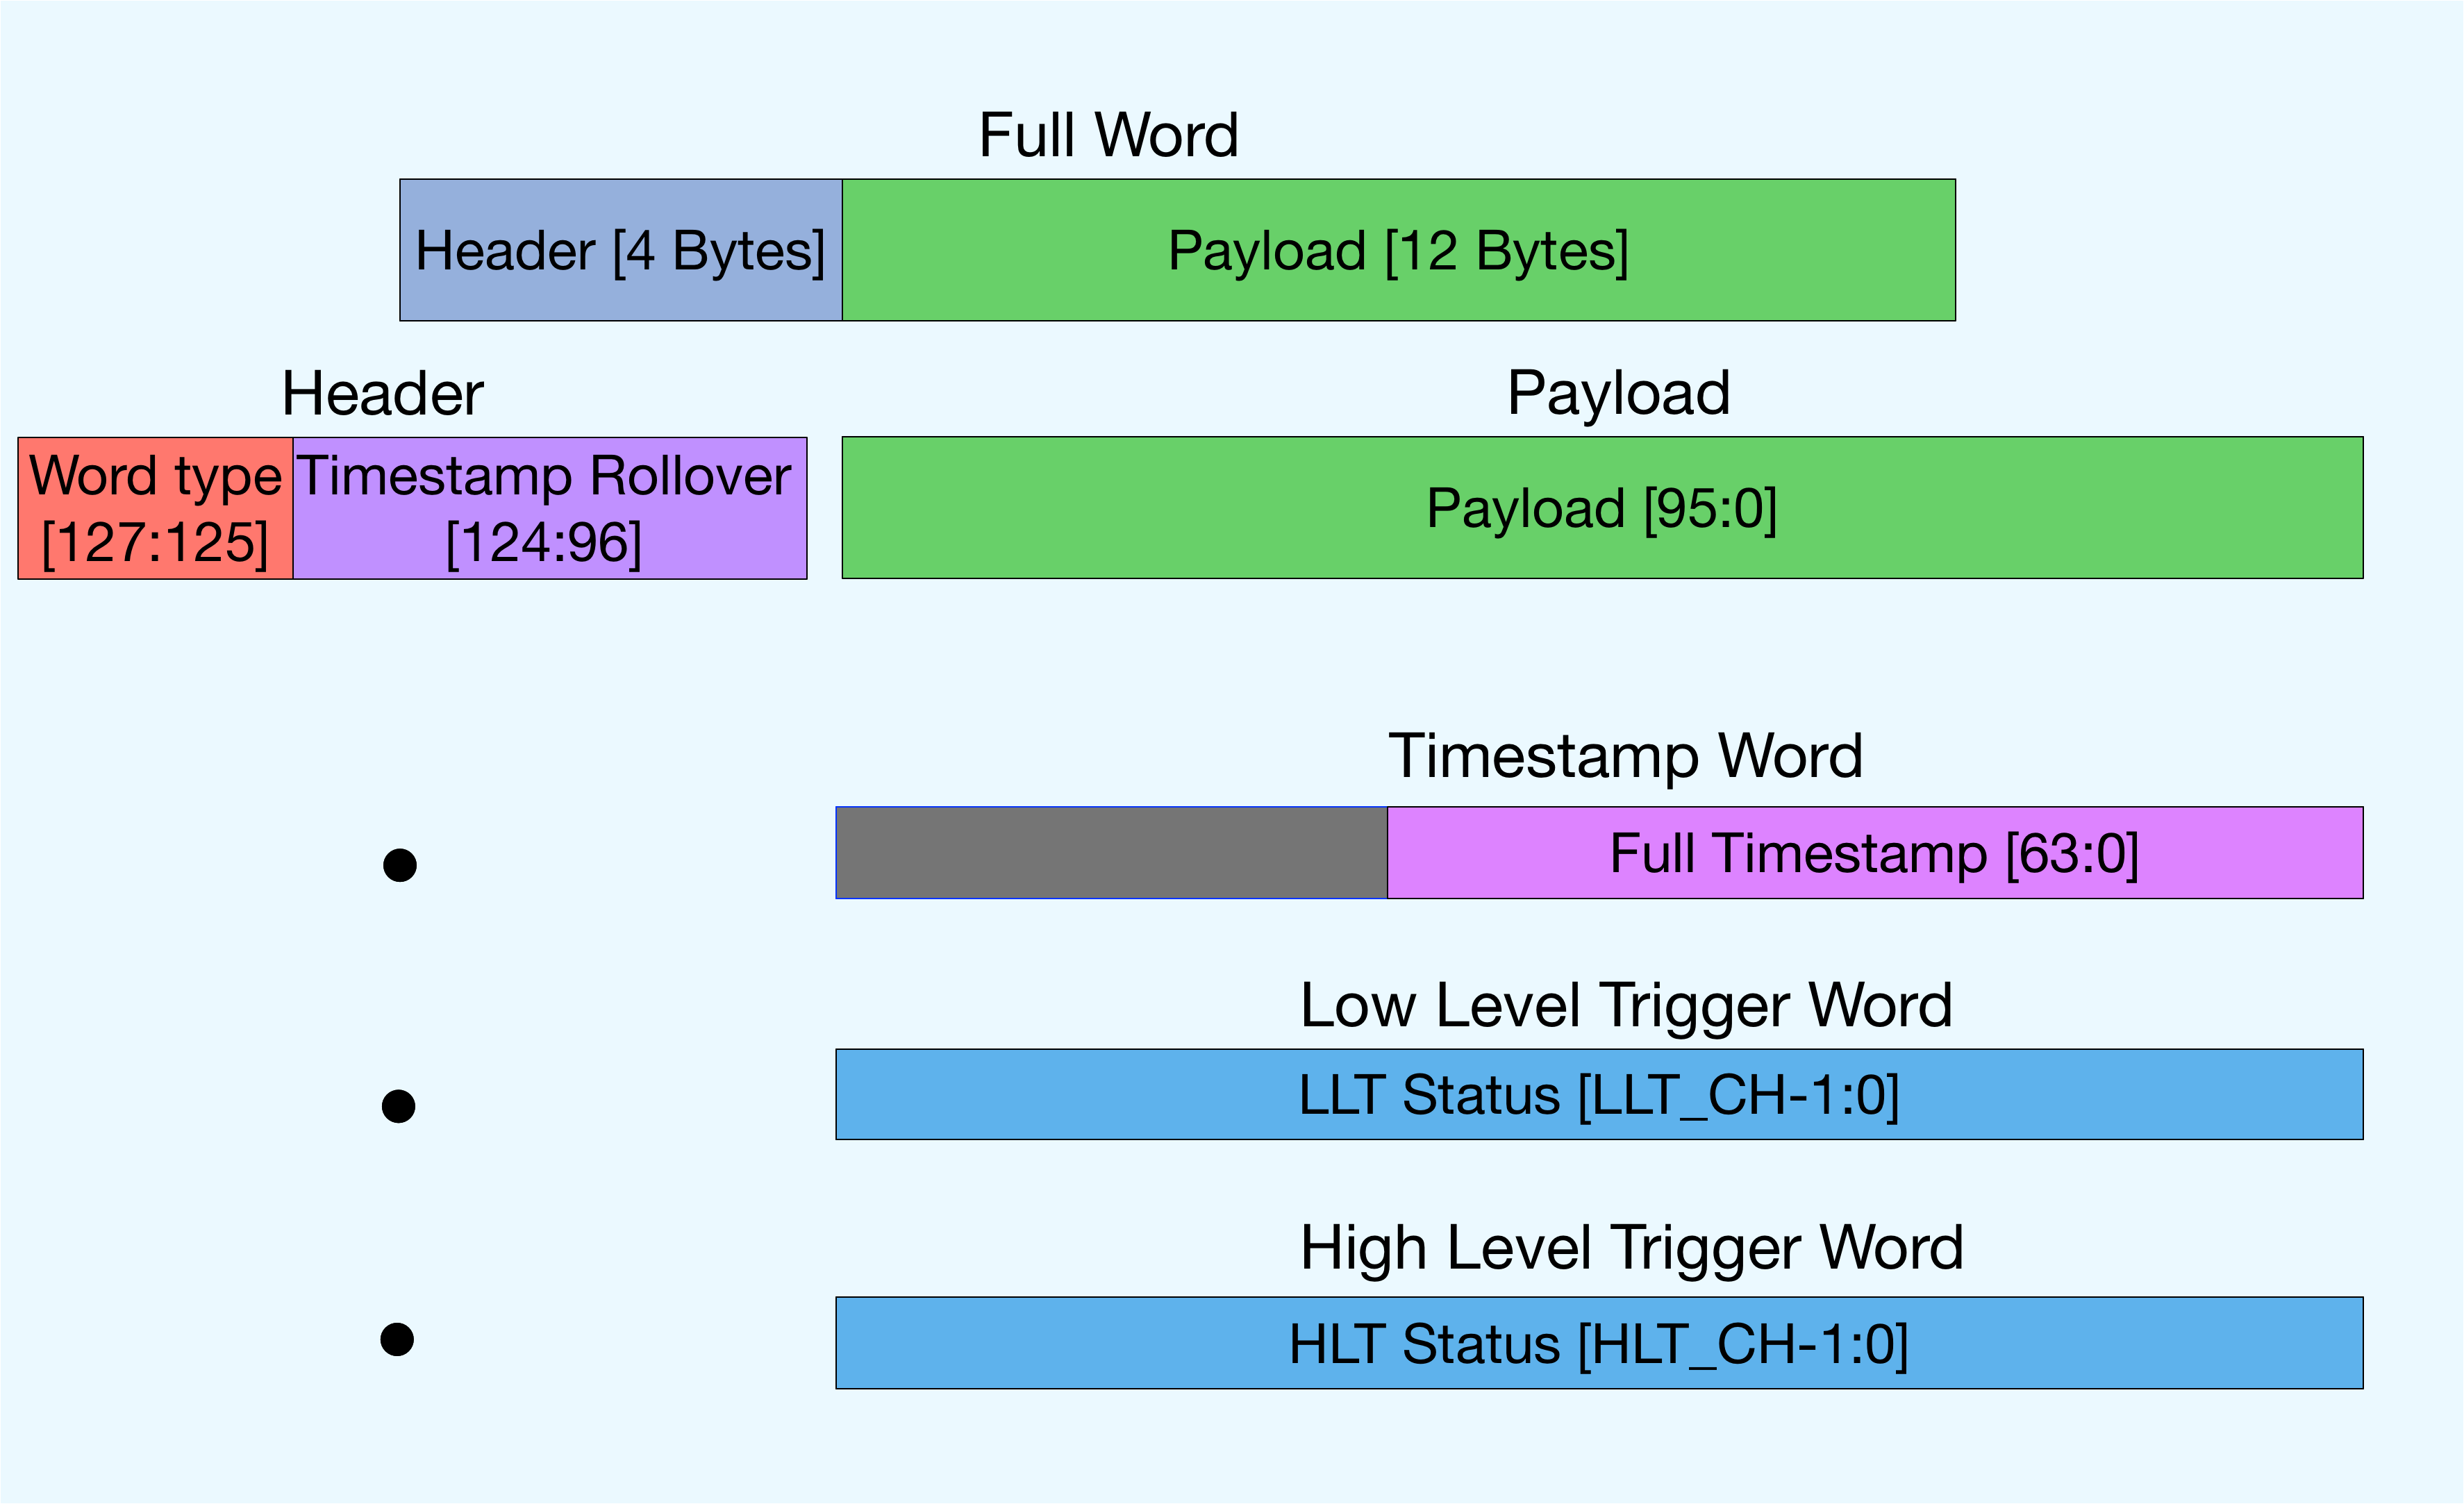
\includegraphics[width=9cm,height=5cm]{figs/fw_word_types_v2_2.png}\\
			\begin{itemize}
				\item[$\bullet$] Format of the data sent from the programmable logic (PL) to processor side (PS).
				\item[$\bullet$] PS Reads out and packages words to be sent to board reader.
				\item[$\bullet$] Timestamp word allows recovery of full timestamp for all words. Always sent before lower 29bit timestamp rollover.
			\end{itemize}
	}
	\frame{  %Page 5
	\frametitle{CTB TCP Packets}
		\framesubtitle{What the board reader recieves }
			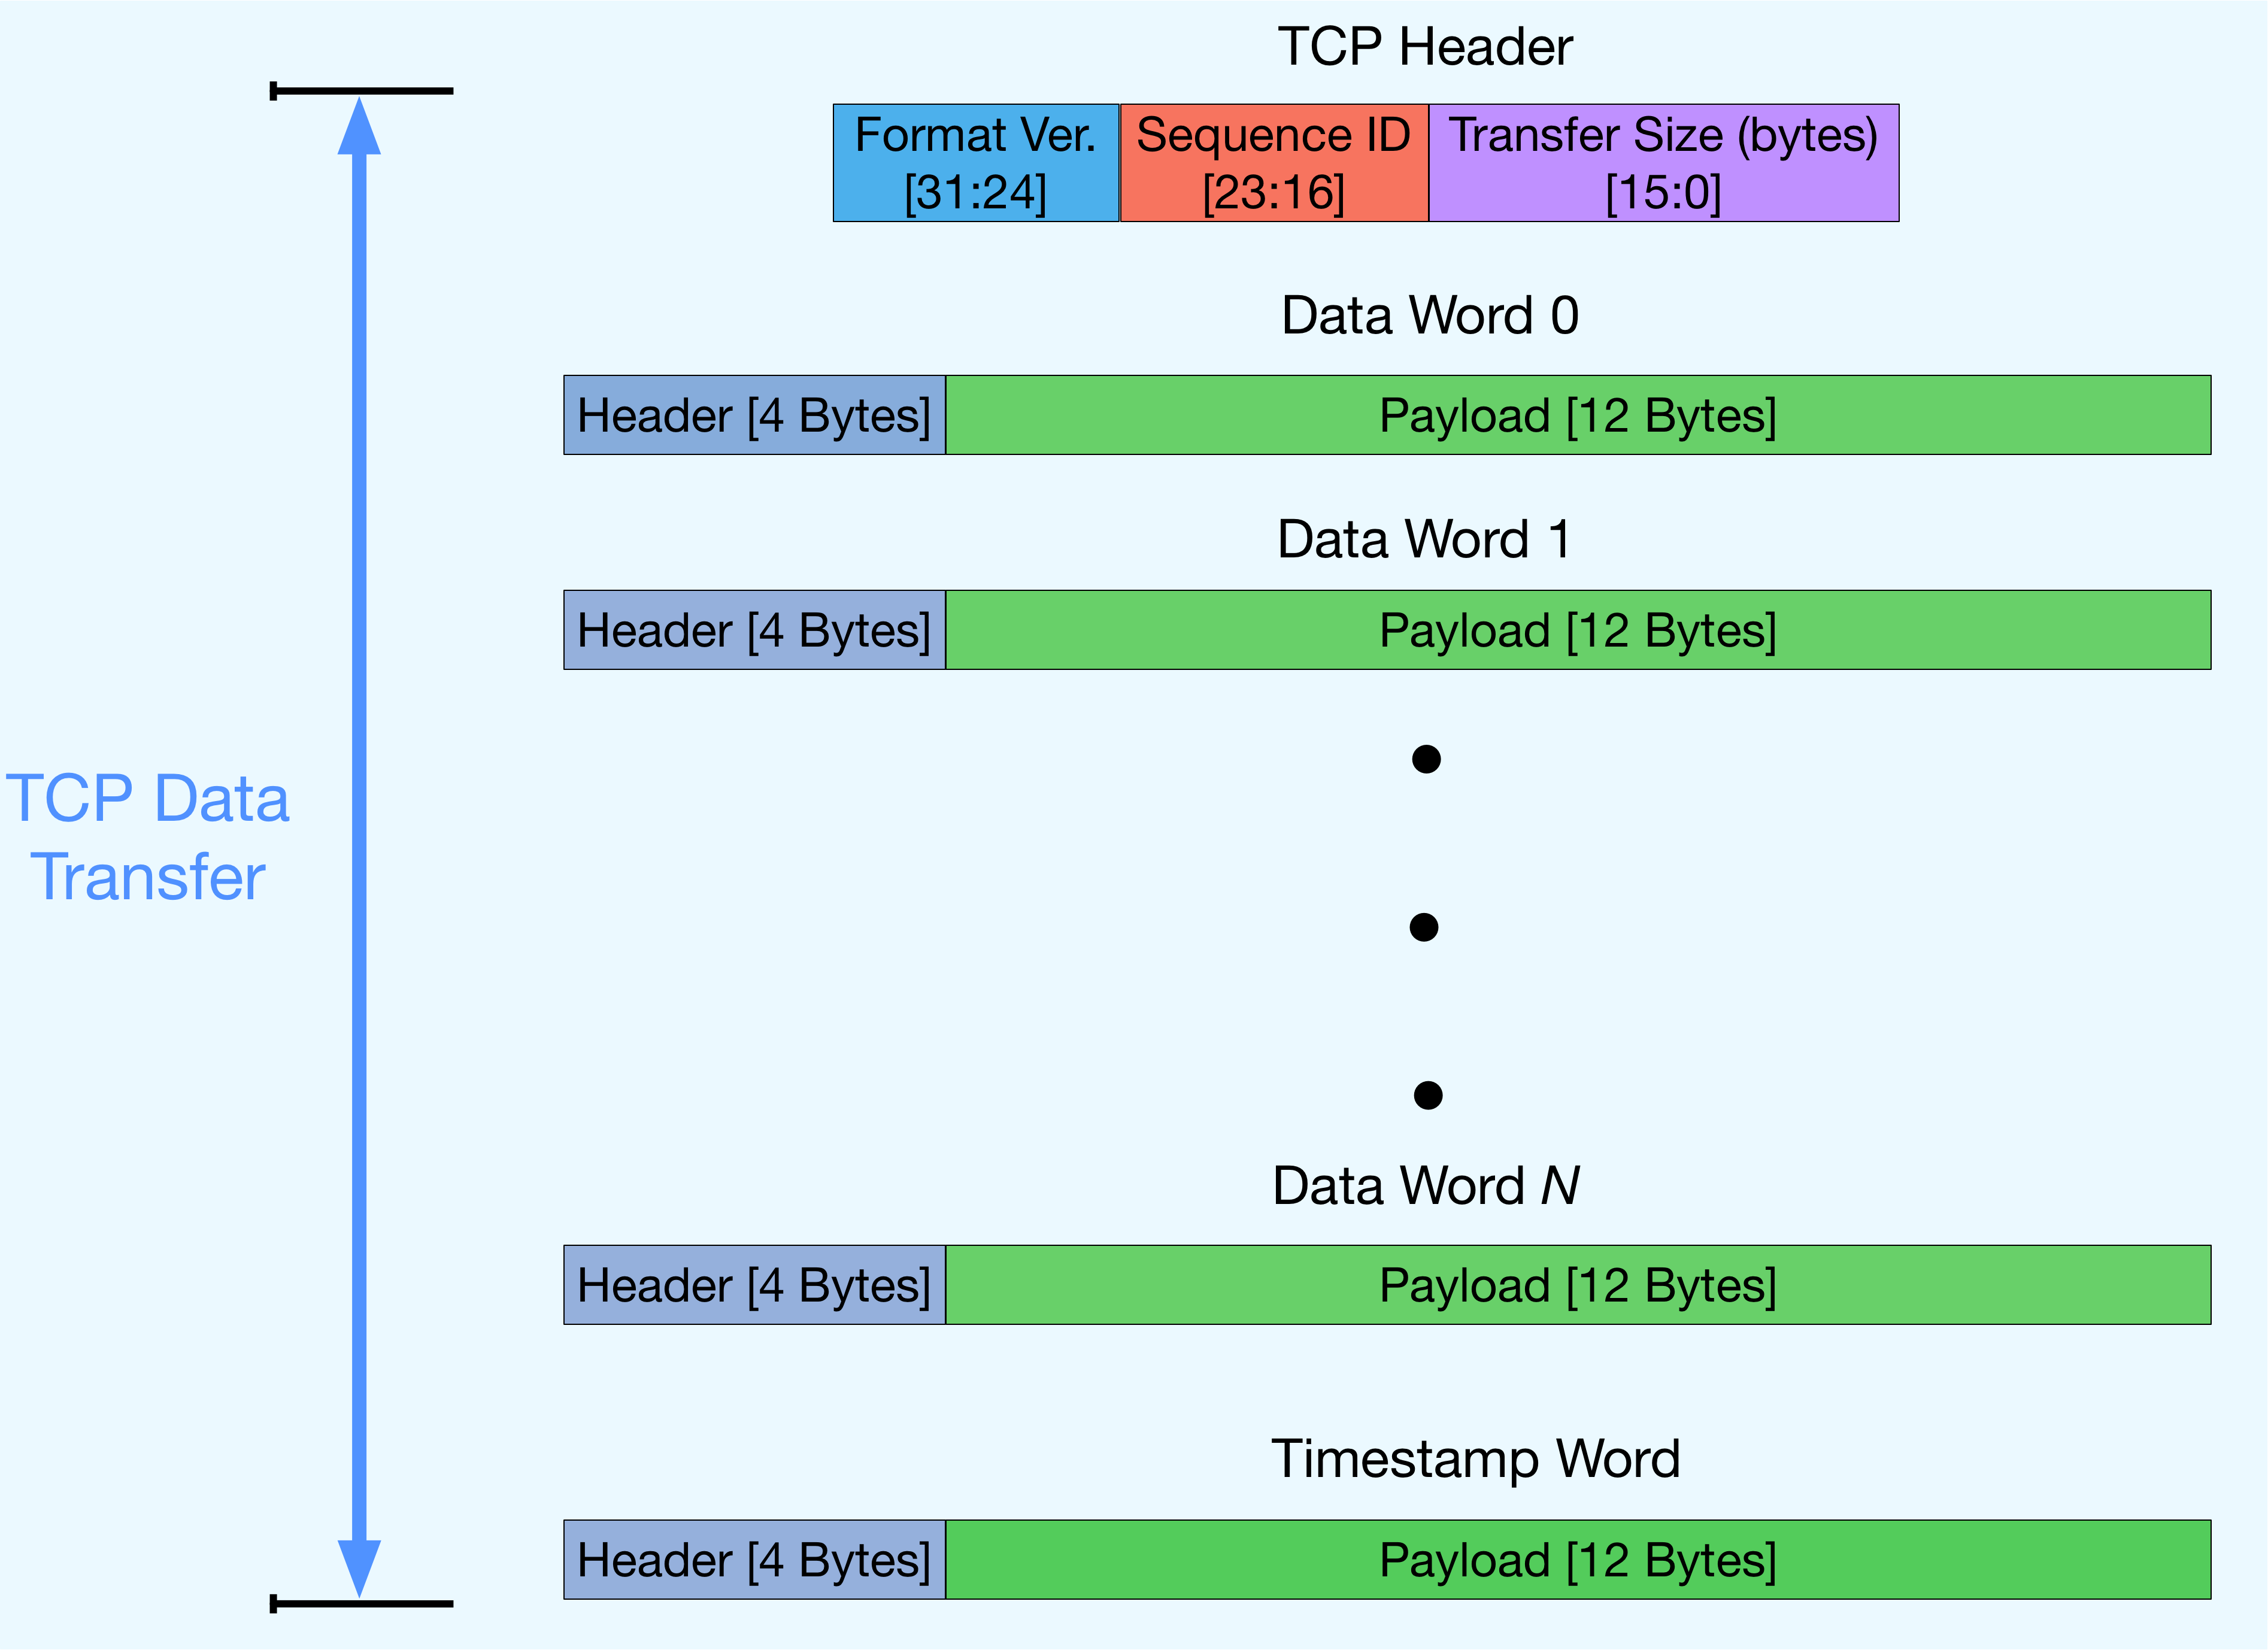
\includegraphics[width=9cm,height=5cm]{figs/fw_tcp_words_2.png}\\
			\begin{itemize}
				\item[$\bullet$] Data recieved by the board reader.
				\item[$\bullet$] Not necessarily what the board reader will write to file. Will need to decide the best format for storing the data.
				\item[$\bullet$] Singe timestamp per transfer and timestamp always ends the data transfer.
			\end{itemize}
	}
	\frame{  %Page 6
	\frametitle{Review Proposed Triggers}
 		\framesubtitle{Nuno's \textit{proposed} triggers and \textit{proposed} order they will be put in place on the CTB}
			\begin{enumerate}
			\item[1. ]  \textcolor{green}{\checkmark} Zero/Minimal bias triggers (commissioning of board and board reader)
			\item[2. ] CRT triggers (to use for commissioning before beam). Ignore beam	instrumentation.
				\begin{itemize}
					\item[$\bullet$] Front-to-back triggers (through-going muons) 
					\item[$\bullet$] Vertical muons (\textit{If} we have top mounted CRT)
			%		\item[$\bullet$] Stopped muons (fire one side of cryostat and not the other)
			%		\item[$\bullet$] Muons through the APA (fire both sides but selecting specific panels to have guaranteed APA crossing) 
				\end{itemize}
			\item[3. ] Triggers with PDS
			\begin{itemize}
				\item[$\bullet$] Mostly to study PDS system in combination with other systems 
			\end{itemize}
				\item[4. ] Beam (un)correlated triggers
				\begin{itemize}
					\item[$\bullet$]  Beam spill (simplest trigger) 
					\item[$\bullet$]  Beam and selection BI detectors (looking for specific beam composition) e.g.,
					\begin{itemize}
						\item[] e$^-$ \hspace{1.05cm}  Chkv1 $\wedge$ Chkv2 \\
						\item[] $\pi$ \hspace{1cm}  $\neg$Chkv1 $\wedge$ Chkv2
						\item[] K/p \hspace{0.64cm} $\neg$Chkv1 $\wedge$ $\neg$ Chkv2
					\end{itemize}
				\end{itemize}
		\end{enumerate}
	}
	\frame{  %Page 7
	\frametitle{Next Steps 1/2}
	\framesubtitle{Integrating more advanced trigger schemes }
	\begin{itemize}
		\item[$\bullet$] We are set up for what we \textit{\textcolor{red}{think}} needs to be done which could be very different from the expectations and/or the reality.
		\begin{itemize}
			\item[$\circ$] The previous slide gives a baseline of trigger schemes, but the priority in which we implement them still needs feedback.
		%	\item[$\circ$] Need more input on the priority of the needed triggers.
			\item[$\circ$] Attempting to make trigger generic enough to handle unforeseen cases. (\textcolor{red}{Does \textit{not} mean we can accommodate anything})
		\end{itemize}
		\item[$\bullet$] Refer to Nuno's slides	\footnote{\href{https://indico.fnal.gov/event/14581/session/8/contribution/141/material/slides/0.pdf}{\textcolor{blue}{Link to full slides}}}
		 for a more in depth look at the trigger schemes. (Note: Some of the content is now obsolete due to subsequent discussions and information.)
		 \item[$\bullet$] \textcolor{red}{To repeat, we must discuss the needed triggers and the possible prescales.}
	\end{itemize}
	}
	\frame{  %Page 8
	\frametitle{Next Steps 2/2}
	\framesubtitle{Integrate subsytems: Beam, CRT, PDS}
	\begin{itemize}
		\item[$\bullet$] Just plug and play, yes? \textit{Never} this easy. :(
		\begin{itemize}
			\item[1. ]  \textcolor{red}{Physically connect subsystems to CTB.}
			\item[2. ] Verify we have a robust connection, e.g., 
			\begin{itemize}
				\item[$\ast$] Use fixed frequency pulse and check recieved signal frequency.
				\item[$\ast$] Timestamp the signal when sent and recieved then compare timestamps offline.
			\end{itemize}
			\item[3. ] Need to calibrate signal delays (\textcolor{red}{very difficult to get right}) from the various subsystems. Suggestions on how we should do this welcomed and needed! Want to avoid the flow below,
			\begin{itemize}		
				\item[1. ] Compare CTB and subsystem timestamps to calculate delay
					\item[2. ] Use trigger \textit{t$_0$} to reconstruct events to check if it makes sense. 
					\item[3. ] Nothing makes sense. . . panic
					\item[4. ] Come up with new plan to calibrate timing.
			\end{itemize}
		\end{itemize}
		\item[$\bullet$] Would like to start integration work in April or May.  
		\begin{itemize}
			\item[$\circ$] Any suggestions of a better time to do this or certain milestones that affect this date?
		\end{itemize}	
	\end{itemize}
	}
	\frame{ %Page 10
	\frametitle{Summary of FW + SW progress}
	\begin{itemize}
		\item[$\bullet$] Firmware progressing.
		\begin{itemize} 
			\item[$\circ$] \textcolor{green}{\checkmark} Version 0 (just timestamps) 
			\item[$\circ$] \textcolor{green}{\checkmark} Version 1 (random triggers) 
			\item[$\circ$] Ongoing - Version 2 (Simple beam gate trigger) 
			\item[$\circ$] Afterwards will follow priorities mentioned before
		\end{itemize}
		\item[$\bullet$] Software on CTB side being improved.
		\begin{itemize}
			\item[$\circ$] Current implementation is working fine, but improvements being introduced
			\item[$\circ$] Need to readjust configuration structure to ProtoDUNE  configuration  needs
			\item[$\circ$]  Introduction of calibration  socket
			\begin{itemize}
					\item[$\ast$]  Calibration is a secondary stream of CTB data (for monitoring purposes)
			\end{itemize}		
		\end{itemize}
		\item[$\bullet$] Board reader.
		\begin{itemize}
			\item[$\circ$]  Able to run in "standalone" mode which means there is a client to receive data from CTB and print or store data on any computer, or more simply put, it is not integrated into artDAQ.
			\item[$\circ$] Would like an update on the board reader status as this is an important link for integrating the trigger into the DAQ system.
		\end{itemize}
	\end{itemize}	
	}
	\frame{ %Page 11
		\frametitle{Summary}
		\begin{itemize}
			\item[$\bullet$] Need continued trigger feedback. Order of trigger implementation, prescales \dots			
			%\item[$\bullet$] Need continued feedback on trigger scheme implementation!
			\item[$\bullet$] Need to start integrating susbsystems soon, to stay on schedule.
			\item[$\bullet$] Ideas welcomed and needed for timing calibrations.
		\end{itemize}
	}

\end{document}